%!TEX root = main.tex

\chapter{Selected criteria to be investigated in this thesis}\label{Chap:selectedCriteria}

In this chapter, firstly, several criteria regarding lateral railway bridge dynamics included in Eurocode EN1991-2 are selected. The reason for the selection is that the selected criteria tend to causing inevitable violation for modern long-span railway bridge designs. 

Then, in order to assess the feasibility and the reliability of the selected criteria, their origin were traced and interpreted. By interpreting the original intension during the creation process of these selected criteria, assessment and remarks can be conducted further on.

Also, within the original research paper, more useful information can be extracted. These information can contribute to further improvement of the criteria or the creation of new validation method.

\section{Selected criteria}

Altogether two criteria were found in EN1991-2 with regard to lateral railway bridge dynamics. They are:

\begin{enumerate}
	\item 1.2Hz Criterion
	\item Nosing force
\end{enumerate}

\subsection{1.2Hz Criterion}
1.2 Hz criterion is defined in \citet[A24.4.2.4]{EC12} with following statement:

\begin{quote}
	...

	\textbf{The first natural frequency of lateral vibration of a span should not be less than $f_{h0}$. The value for $f_{h0}$ may be defined in the National Annex. The recommended value is: $f_{h0}=1.2 Hz$}

	...

\end{quote}

This criteria rejects almost all bridge designs that have span longer than 150m. This is due to the reason that longer span bridges possess lower lateral natural frequency. When the span is over 150m, normally the lateral natural frequency of the bridge fall below 1.2Hz. 

\subsection{Nosing force}\label{sec:nosingforce}
Nosing force is defined in Eurocode 1991-2. 

The characteristic value of the nosing force shall be taken as $Q_{sk} = 100kN$. It shall not be multiplied by the factor $\Phi$ (\citet[6.45]{EC12}) or by the factor $f$ in \citet[6.51]{EC12}. 

The characteristic value of the nosing force should be multiplied by the factor $\alpha$ in accordance with \citet[6.3.2]{EC12} for values of $\alpha \geq 1$

The nosing force shall always be combined with a vertical traffic load.


\subsection{Origins of selected criteria}
The selected criteria shares the same original research project conducted by ERRI(former UIC). The project is called: \textit{D181: Lateral forces on railway bridges}. 

\paragraph{Origin of 1.2Hz Criterion}
Its original proposal can be found in \citet[Proposed criteria]{d181}. The evidence of the this statement is that both definition use almost the same language. The original one explained the reason for choosing 1.2Hz frequency but EN1991-2 omitted the reason for choosing. The original definition is extracted as following for reference:

\begin{quote}
	To avoid the occurrence of resonance in the lateral motion of the vehicles due to the lateral motion of the bridge, a limit value lower than the first natural frequency $f_1t$ of the lateral vibration of the span studied should be fixed. The natural frequency for lateral movements is between 0.5 and 0.7 Hz for coaches and between 0.7 and 1 Hz for locomotives. We therefore propose a safety margin $F_{lt} \geq 1.2Hz$
\end{quote}

\paragraph{Origin of nosing force}
Its original background can be found in \citet[Proposed criteria]{d181}. It is defined as a representation of actions, in combine with actions like vertical loads, dynamic effects, centrifugal forces, traction and braking forces, etc.

The evidence of RP6 is the background of nosing force in EN1991-2 is the following repeating literature:

In \citet[6.5.2]{EC12}:
\begin{quote}
	(1)P The nosing force shall be taken as a concentrated force acting horizontally, at the top of the rails, perpendicular to the centre-line of track. It shall be applied on both straight track....
\end{quote}

In \citet[4.1B]{d181}:
\begin{quote}
	These forces shall be applied at the top of the rails in the most unfavourable position and acting horizontally, perpendicular to the track centreline...
\end{quote}

With another statement also helps proofing RP6 is the background of nosing force in EN1991-2 in \citet[4:Draft Recommendations]{d181}:

\begin{quote}
	These can therefore be expressed as follows: (Article \textbf{6.5.2} of ENV 1991-3 of 1994)...
\end{quote}

ENV 1991-3 was renamed to EN 1991-2 in 2003.

Originally in \citet[4:Draft Recommendations]{d181}, nosing forces was defined as lateral forces from vehicle/bridge interaction as a result of \textbf{hunting}.

\section{Conclusion}
Since all criteria regarding lateral railway bridge dynamics come from the same research project: \textit{D181:Lateral Forces on Railway Bridges}, it's essential to interpret the whole report series in order to have a better understanding on its proposed criteria. Next chapter will lay emphasis on interpreting and in the end, conduct assessment on the criteria.


\chapter{Evaluation on the supporting research of the selected criteria: D181 research}\label{sec:D181reportseries}


\section{Introduction}

This chapter aims to interpret several key documents within the research report series D181. The investigated documents contains relative contents to the problem-causing criteria filtered out already in Chapter.\ref{Chap:selectedCriteria}.

D181 Committee Group is created by UIC, in order to investigate Lateral Forces on Railway Bridges. Some of the proposed criteria in reports created by this committee group are adopted by Eurocode Committee to created Eurocode 1991-2. The goal of this interpretation is to summarize the research done by D181 report series and and give further conclusion.

The interpretation will be done in following aspects:

\begin{enumerate}
    \item Interpretation of DT329
    \item Interpretation of RP6
    \item Conclusion of D181 report series
\end{enumerate}

In this thesis document DT 329 and document RP 6 are obtained and studied, but other reports in English version are not available to the researcher.
For an overview of structure of report series, please refer to Appendix.\ref{app:generalInformationD181}.

\section{Items of interests in report series}

\begin{enumerate}
    \item Resonance mechanisms studied. They are discussed in DT329. See Section.\ref{sec:resonance329}
    \item The proposed 1.2 Hz Criterion and its background. It is discussed in RP6. See Section.\ref{sec:1.2criterion329}
    \item  Lateral forces(Nosing force) on the bridges. See Section.\ref{sec:lateralforce329}
\end{enumerate}


\section{Methodology of Parametric Research DT329}

The DT329 research was conducted in two phases. It is noted that all studies were done using VAMPIRE software. The reliability of simulation has been discussed and confirmed in a previous report of \citet{d181rp2}.

In the initial phase 11 sets of bridge parameters were selected for the simulation. 52 combinations of bridge parameters and train configurations were examined. The goal of the initial phase is to filter out most influencing parameters for bridge dynamics.

In the secondary phase, the influence of selected parameters were categorized into 3 cases. They include:
\begin{enumerate}
 \item the influence of multiple span bridges (viaducts)
 \item the influence of track quality
 \item the influence of stiffness/span/frequency on the resonant behaviour of the bridge
\end{enumerate}
They were studied by using the same simulation method used in initial research phase.


\begin{figure}[h]
\centering
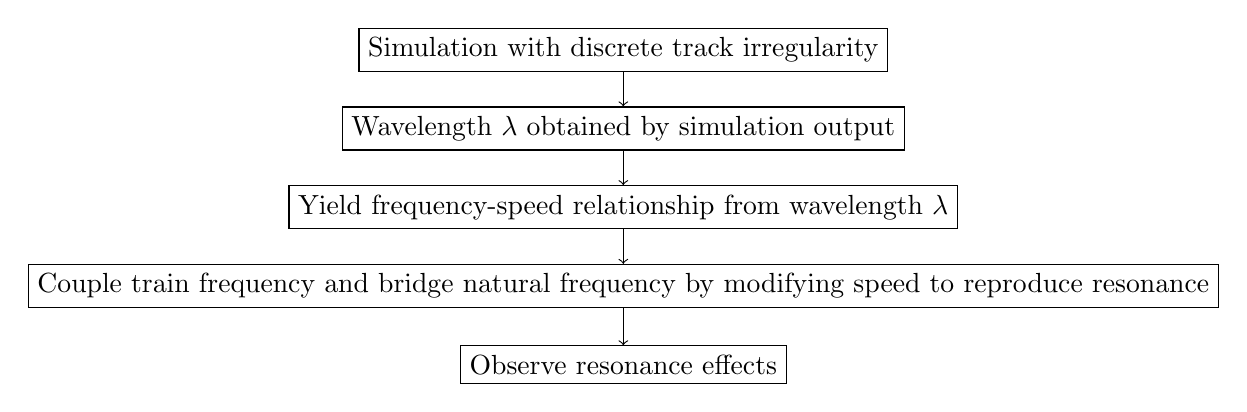
\begin{tikzpicture}
    \node[draw] (simulation1) at (0, 0) {Simulation with discrete track irregularity};

    \node[draw] (analysis) at (0, -1) {Wavelength $\lambda$ obtained by simulation output};

    \node[draw] (yielding) at (0, -2) {Yield frequency-speed relationship from wavelength $\lambda$};

    \node[draw] (matching) at (0,-3) {Couple train frequency and bridge natural frequency by modifying speed to reproduce resonance};

    \node[draw] (observe) at (0, -4) {Observe resonance effects};

    \draw[->] (simulation1) to (analysis);

    \draw[->] (analysis) to (yielding);

    \draw[->] (yielding) to (matching);

    \draw[->] (matching) to (observe);
\end{tikzpicture}
\caption{Workflow of kinematic resonance research}
\label{fig:workflow329kinematic}
\end{figure}


\section{Interpretation of resonance phenomenon studied in DT329}\label{sec:resonance329}

2 types of resonance were studied in DT329, including:

\begin{enumerate}
    \item Resonance caused by axle repeat pattern
    \item Resonance caused by kinematic movement
\end{enumerate}

Frequency shift phenomenon is an important characteristics observed from resonance effects lists above. It is explained in Section \ref{sec:apparentshift}

\subsection{Mechanism of resonance caused by axle repeat pattern}

In \citet[3.4.3]{d181dt329}, explanation on the mechanism of such resonance is explained as following:

\begin{quote}
    Axle repeat patterns are wavelength phenomena - regardless of vehicle speed, the repeat length is constant. However, since frequency is speed divided by wavelength, the frequency of the axle repeat patterns vary with train speed. A table of axle repeat pattern lengths, and typical frequencies arising from train speed are given in Figure.\ref{tab:329axlerepeat}

    By running train at different speeds shows resonance is possible between train and bridge if the axle passing frequency coincides with the first lateral bridge mode. The effect occurring in bridge lateral displacement over a limited frequency range around the resonance frequency.
\end{quote}



However, the speed on theory which should yield resonance effect may be different from the speed that actually triggered resonance.

\subsection{Mechanism of resonance caused by kinematic movement of trains} 

In \citet[3.4.3]{d181dt329}, explanation on the mechanism of such resonance is explained as following:

\begin{quote}
Kinematic wavelength also gives rise to frequencies which vary with speed for the same reason. For first lateral bending mode coincidence with kinematic frequency, the kinematic wavelength of each train type had to be established, by running each train at a range of typical operating speeds over a discrete lateral irregularity, and examining the frequency content of the lateral wheel motion. The resulting wavelength ranges are tabulated in Table.\ref{tab:329kinematicwavelength}. See Figure \ref{fig:workflow329kinematic} for an overview of workflow of this study.

The most likely possible resonance in the initial studies to be of this type was between the passenger train at 200 km/h (55.556 m/s) on passenger track and BR PI wheel profiles, and a span of 54 m, stiffness 1/10000, mass/length of 6 tonnes/m. This combination was examined by varying the speed between 55.556 - 64.6 m/s over the span, and by varying the stiffness of the span between 117000 and 1112000 running the train at 55.556 m/s. Another combination was examined - the ETR500 train running between 65 - 80 m/s on high speed track and BR PI wheel profiles, for a span of 38 m, stiffness 1110000, and mass/length 10 tonne/m; the span in this case was chosen to coincide with the kinematic wavelength of the coaches.

Coincidence of vehicle kinematic frequency with bridge first lateral bending mode may cause resonance to occur over a broad range of frequencies to a less pronounced effect than coincidence of axle passing frequencies. Evidence of coincidence of kinematic wavelength with length of span has been found in the lateral acceleration of bridges, but was not demonstrated in the lateral bridge displacement in the cases examined. For short kinematic wavelengths, this effect could not be seen, possibly because of lack of time for the bridge to respond.

\end{quote}


\subsection{Apparent shift in resonance frequency}\label{sec:apparentshift}
It is frequently observed in the output of both resonance effects that apparent resonance happens at some frequencies higher than frequencies calculated on theory. This is explained in following quote on \citet[Page 13, Secondary Phase]{d181dt329}. However, the explanation wasn't verified by further studies. They can only be treated as hypothesis.

\begin{quote}
Although the peak mid span displacement was expected to occur at 28.5 mis, it can be seen that for the runs with just the coaches that the peak occurs at about 32 m/s. This is confirmed to be a resonance-type effect rather than a discrete event in the time histories of the runs, a selection of which are shown in Figure C6(Original report), of which an extract of 100-285m follows as Figure C7(Original report). This speed is mid way between axle passing frequency coinciding with first bending mode of the bridge, and kinematic frequency coinciding with the first bending mode. So, the apparent shift in resonant frequency may be due to a combination of these effects (see discussion of kinematic frequency resonance results). However, an alternative explanation may be that as track forces generally increase with speed, the deflection of the span would be expected to increase. If this effect continued through a resonant band, the peak displacement would appear greater at a speed slightly above that calculated for resonance, as sketched in Figure \ref{fig:apparentshift}.
\end{quote}

\begin{figure}[h]
    \centering
    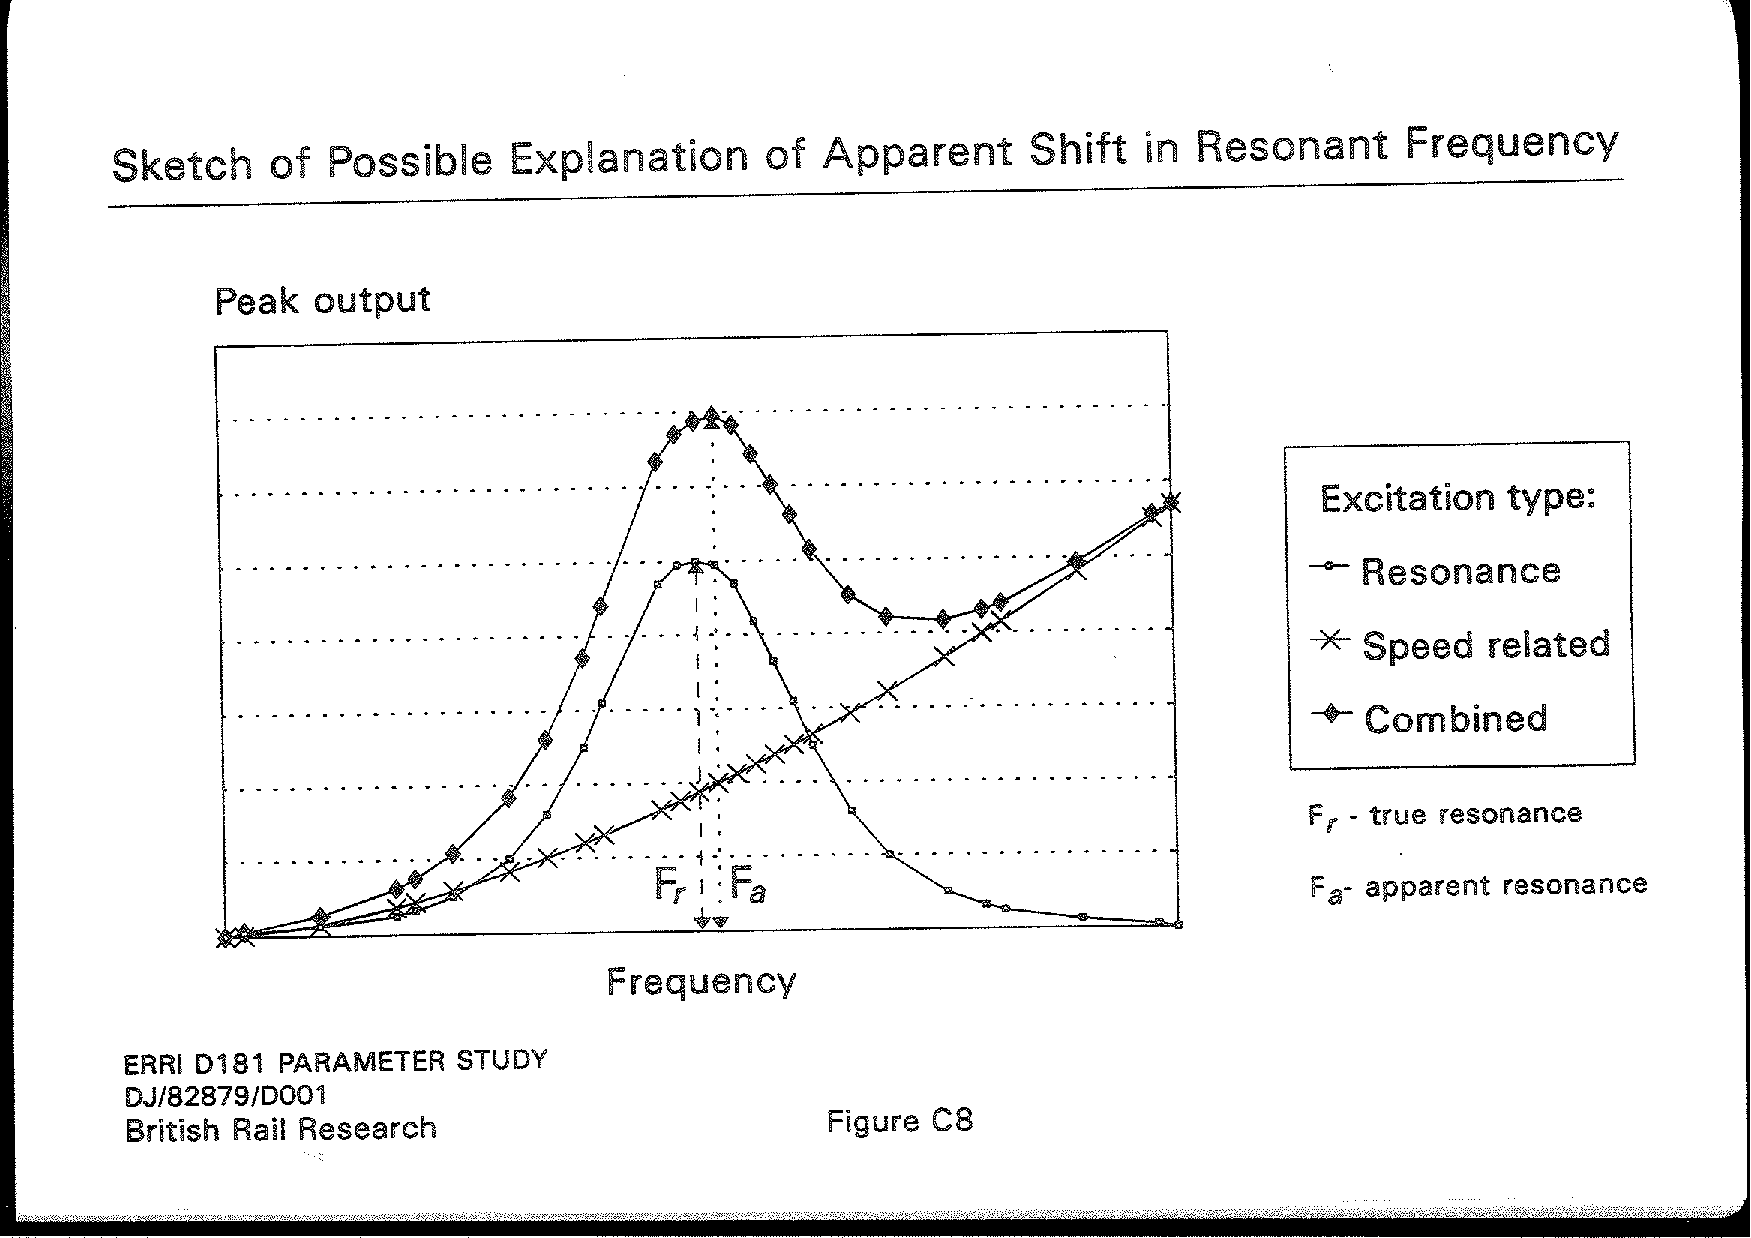
\includegraphics[width=\textwidth]{apparentshift}
    \caption{Sketch of Possible Explanation for Apparent Shift in Resonant Frequency. Extract from \citet[Appendix 2]{d181dt329}}
    \label{fig:apparentshift}
\end{figure}

In the sketch of possible explanation of apparent shift in resonant frequency(Figure \ref{fig:apparentshift}), the combined effect is the superposition of both resonance effect and speed-related effect. Speed-related effect simply increase when speed increase regardless of resonance. Speed is linear to frequency. Thus speed-related effect also simply increase when frequency increases. Resonance effect has an impact where frequency of train and bridge coincides. Speed-related effects is the cause for the frequency shift of combined peak output.

Both explanations indicate that apparent resonance frequency can hardly be predicted. Apparent frequency may even shift into domain lower than theory frequency. 


\section{Investigation of RP6}

\subsection{Debate on proposed 1.2Hz criterion}\label{sec:1.2criterion329}

The value of frequency limit, 1.2Hz is explained in \citet[p3.2: Criterion 2]{d181}:

\begin{quote}
To avoid the occurrence of resonance in the lateral motion of the vehicles due to the lateral motion of the bridge, a limit value lower than the first natural frequency $f_1t$ of the lateral vibration of the span studied should be fixed. The natural frequency for lateral movements is between 0.5 and 0.7 Hz for coaches and between 0.7 and 1 Hz for locomotives. We therefore propose a safety margin $F_{lt} \geq 1.2Hz$

\end{quote}

The original author of report RP6, mr.Graham Scott, was contacted to reveal the background of 'natural frequency for lateral movements'. Mr.Scott is still in charge of the development of software VAMPIRE and he's still active in the field. Unfortunately he was unable to remember what did 'natural frequency for lateral movements' stand for in previous quotes since it was written nearly 20 years ago. He passed me to his colleague Alan Minnis for further questions. Mr.Minnis stated following:

\begin{quote}
Looking at the values I think they would refer to typical rigid body modes of a vehicle.  These are independent of speed and a typical passenger coach with air suspension will have a lower sway frequency of around 0.6Hz which is within 0.5-0.7Hz.  Locomotives tend to have a slightly stiffer suspension hence the slightly higher frequency range.
\end{quote}

Mr.Minnis statements, combined with results yielded in supporting parametric report DT329 proves 1.2Hz criterion is aiming to avoid occurrence of resonance. But this \textbf{isn't} a feasible strategy for the following reasons:

\begin{enumerate} 
    \item The resonance between rigid body mode of train and first lateral vibration mode of the bridge has never been discussed in all D181 report series. No research proofed this kind of resonance can be critical in real life scenario.

    \item There are lots of evidence can be found in report DT329, showing resonance can happen on a bridge with a first lateral natural frequency even higher than 1.2Hz, which is self-conflicting with 1.2Hz criterion. In fact, the resonance could happen at any frequency on theory. For example, \citet[Page 14,Phase II]{d181dt329} shows resonance occurs on 1.71Hz:
        \begin{quote}
            The first lateral bending mode of this bridge is at 1. 71 Hz. The kinematic wavelength of the passenger coaches is around 34-38 m, giving a kinematic frequency range of 1.46 - 1.63Hz.Speeds of 58.14 m/s(1.53-1.71 Hz)and 64.6m/s(1.7-1.9Hz)were also done. The mid span lateral displacement for each of the time histories are shown in Figure C12(Orignial report). The slowest speed appears to show the greatest resonance.
        \end{quote}
\end{enumerate}

\subsection{A new lateral force model based on RP6 simulation results}\label{sec:lateralforce329}

\subsubsection{Basic characteristics of lateral force on railway bridges}
It is concluded in initial phase of the study that presence of the bridge doesn't influence the track forces and track quality is a major factor in determining the lateral forces generated by a particular train on \citet[Page 7, Secondary Phase]{d181dt329}



\begin{quote}
    From the initial study [1], it was concluded that the track quality on a bridge is a major factor in determining the lateral forces generated by a particular train. The D181 Committee therefore asked BRR to determine the peak track forces generated over a wide range of track qualities.

    The length of a bridge is small compared to the overall length of a railway track and so track quality on a single bridge may not be representative of that on other bridges on the same route. However the initial study concluded that, in general, the lateral track forces are not influenced by the presence of the bridge.
\end{quote}

The resonance effects mentioned in the previous sections were only observed in deflection and acceleration domain due to the reason that the presence of the bridge doesn't influence the track forces. 


Influence on the total lateral force as a result of hunting of single vehicle bodies were examined. Three parameters were involved in this parametric research. They were vehicle speed, track irregularities deviation and wheel conicity.

Vehicle speed plays a key role. When speed is 60 km/h for freight trains, in the response output, there is very limited influence by increasing both track deviation and conicity. Different conicity tends to yield same force output. Same as track deviation. See Figure.\ref{fig:b1}.

\begin{figure}[h!]
    \centering
    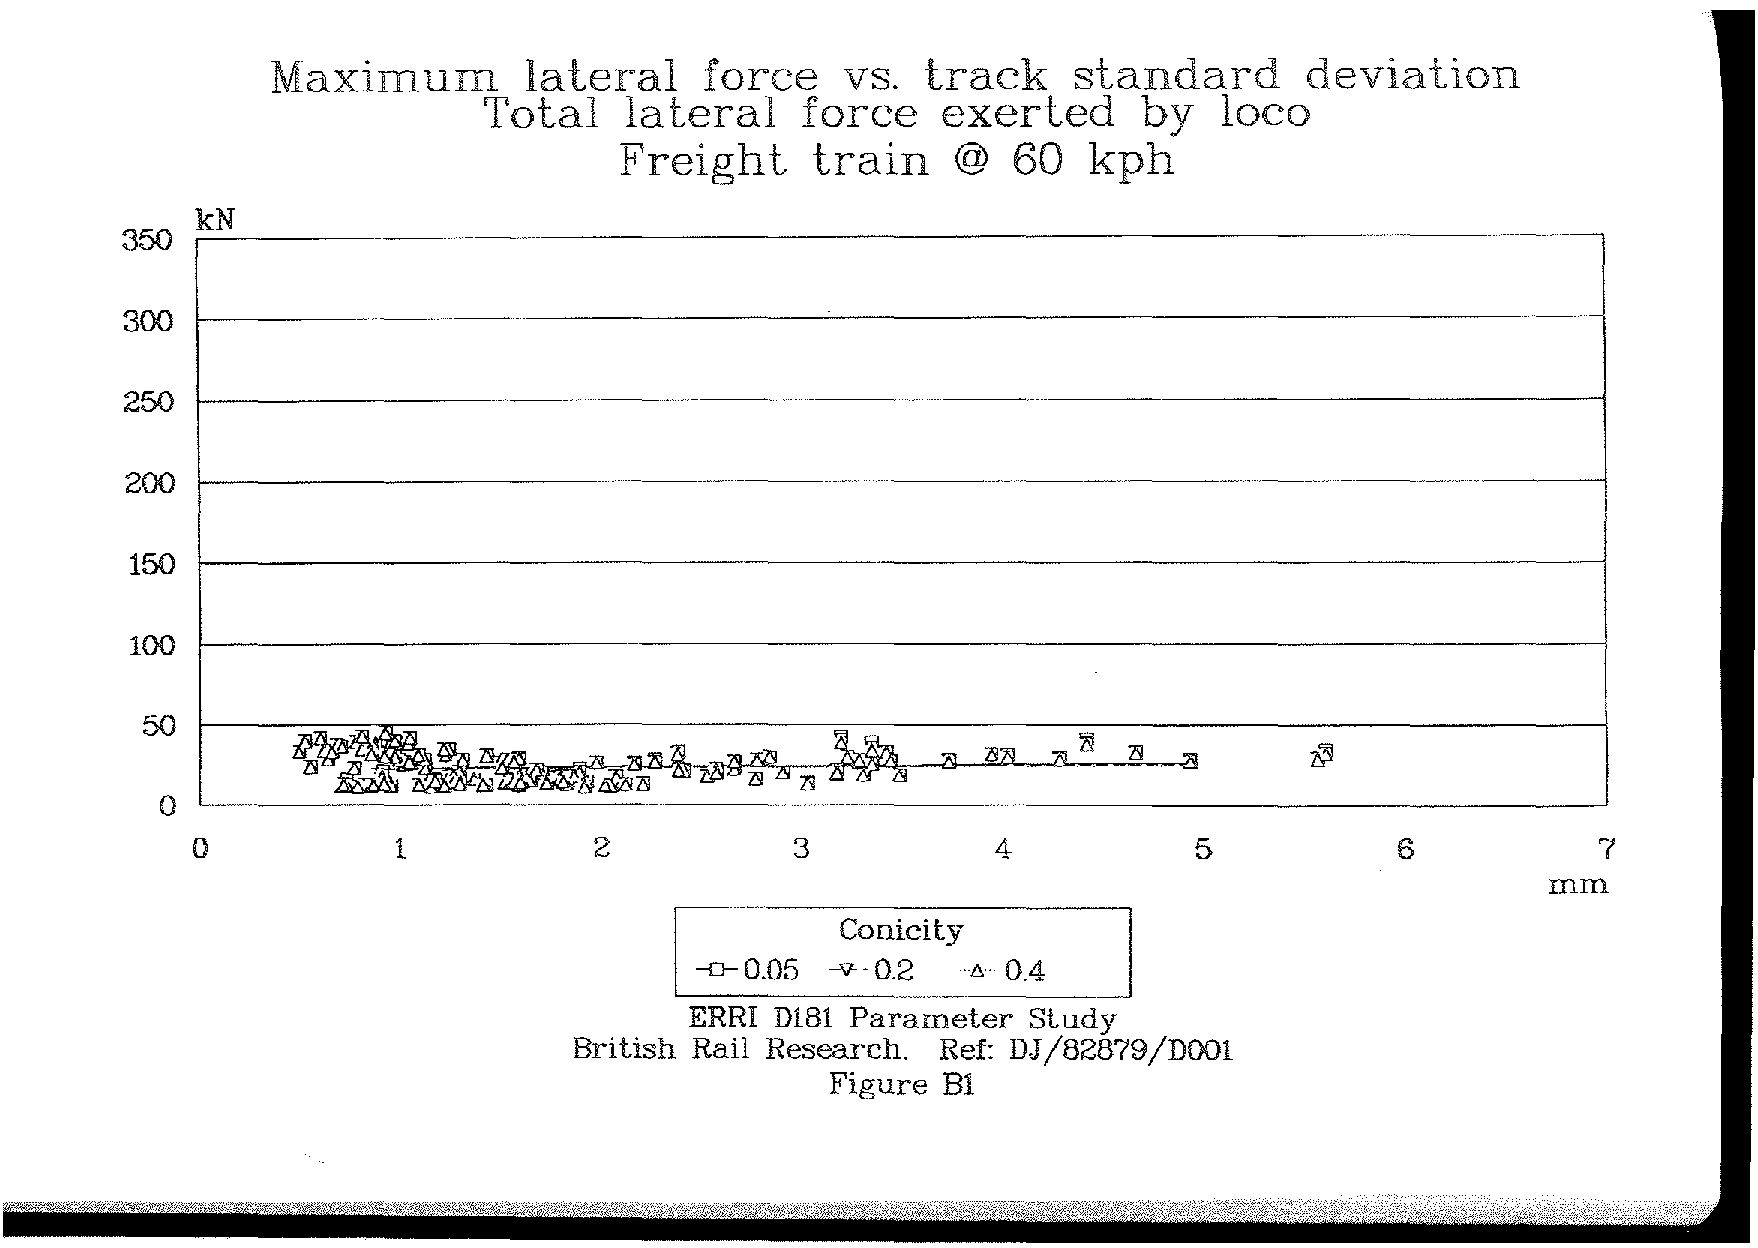
\includegraphics[width=0.8\textwidth]{b1}
    \caption{Figure B1 extracted from \citet{d181dt329}}
    \label{fig:b1}
\end{figure}


When speed increases, output of different conicity on same track deviation is more scattered. Similarly, increased deviation yields yields greater output. They are two basic trends observed in all output data.

However, it is uncertain which conicity will yield greater output compared to other 2 conicity setups. Surprisingly, in some cases, best maintained wheel profile (effective conicity 0.05) generates greater output than poorly maintained wheels (effective conicity 0.4). See Figure.\ref{fig:b2}. The most obvious case of this kind is freight train running at 100 km/h on track with 5.7mm (approximate) deviation.

\begin{figure}[h!]
    \centering
    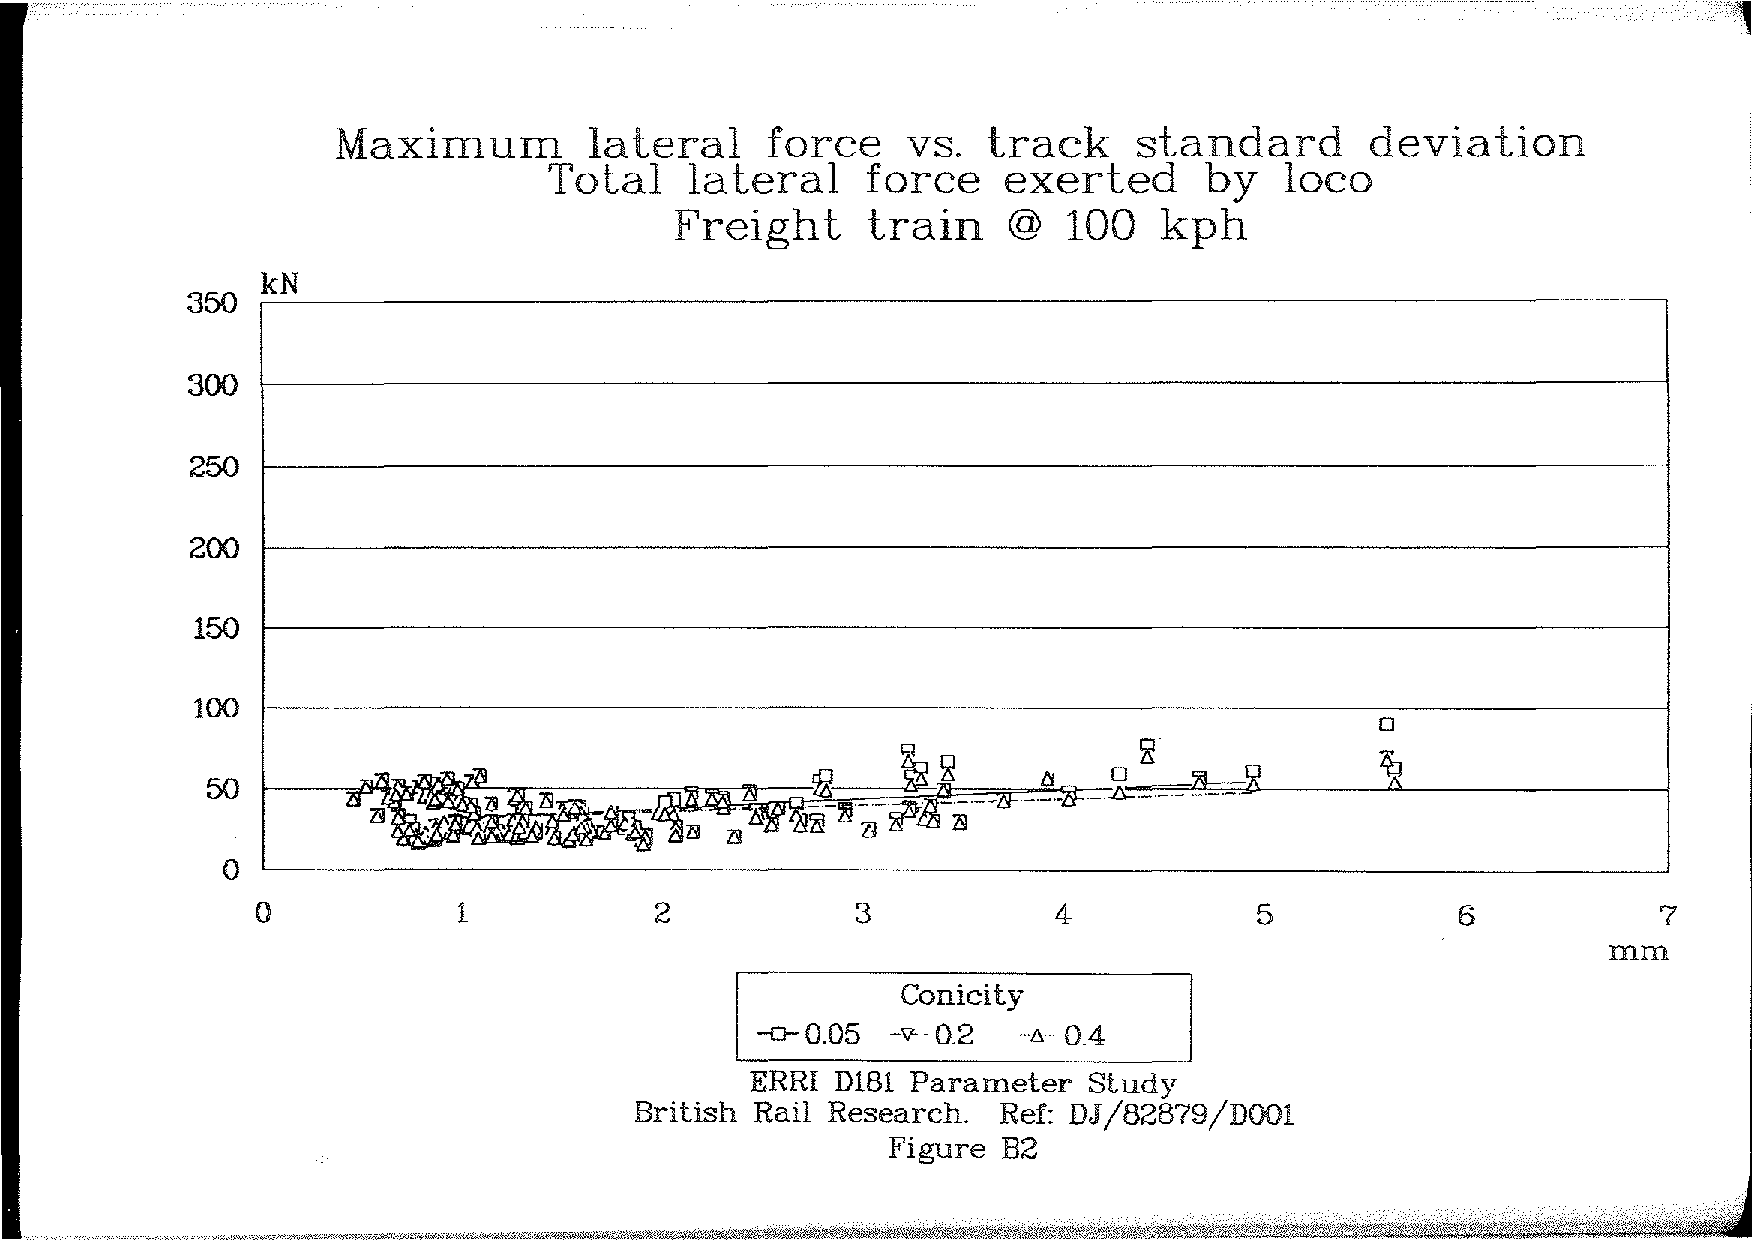
\includegraphics[width=0.8\textwidth]{b2}
    \caption{Figure B2 extracted from \citet{d181dt329}}
    \label{fig:b2}
\end{figure}

Different from conicity, the influence of increasing track deviation is simply predictable. Research report DT329 provided an approximate linear function for relationship between lateral force and track deviation. These linear functions can be extracted from plots B1-B30 of DT329.

Since peak force output of 120 km/h freight train and 200 km/h passenger train are close(2\% difference), it is reasonable to conclude that passenger train tends to yield smaller result than freight train at same speed. This is probably due to passenger trains have more sophisticated suspension system designed to suppress lateral motion of the vehicle. Unfortunately, only one speed of 200km/h configuration was available in DT329. But since freight train yields greater output, it is conservative for designer to adopt force output of freight trains for speeds of 60km/h, 100km/h, 120km/h.

It is worthy to point out a suspicious mistake of DT329 in Table.\ref{tab:peaklateralforce}. Report claimed that output data were filtered by statistical analysis. The peak lateral track force was determined from a statistical analysis of lateral track forces as $M \pm 3\sigma$ where $M$ is the mean lateral force value over the segment and $\sigma$ is the standard deviation over the segment. It does not give a true maximum lateral force but on which is greater than 99.5\% of all force values. It is obvious in Table.\ref{tab:peaklateralforce} that output data of 160kN for freight train wagon was not filtered by statistical analysis. It is the greatest value among all raw output data of freight train running at 100 km/h. See Figure.\ref{fig:b7}. This data of 160kN also illustrates that 
peak forces will be influenced by discrete features in the track geometry which may not be reflected thoroughly in the standard deviation. This thesis report suggest substitute 160kN with 80kN(value by approximate observation). See Table.[note1]\ref{tab:peaklateralforce}

\begin{figure}[h!]
    \centering
    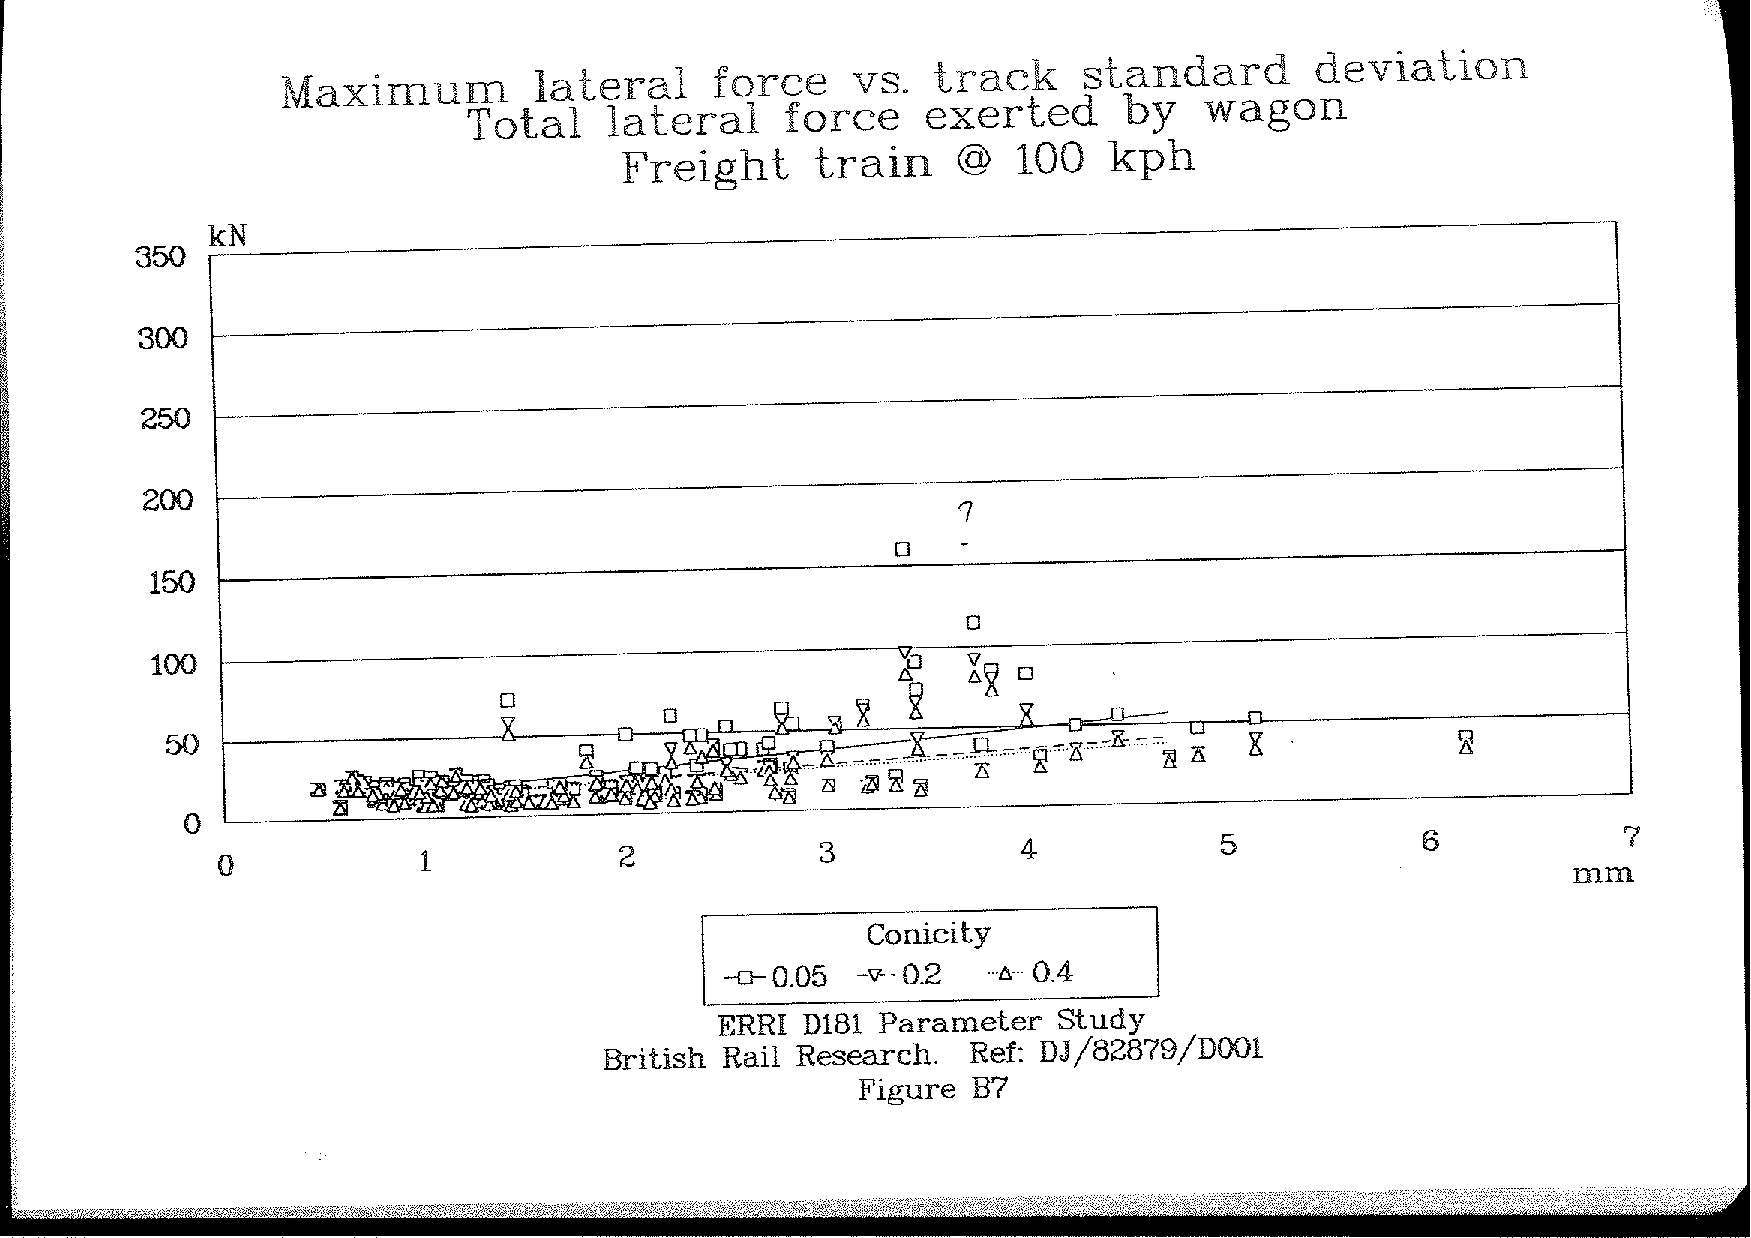
\includegraphics[width=0.8\textwidth]{b7}
    \caption{Figure B7 extracted from \citet{d181dt329}}
    \label{fig:b7}
\end{figure}

\begin{table}[h!]
    \centering
    \caption{Peak Lateral Track Force Over All Track Qualities. Extracted From \citet[Tab. B1]{d181dt329}}
    \begin{tabular}{cccc}
        \hline
        Peak lateral force(kN) & Locomotive Total & Coach/Wagon & Total \\ 
        \hline
        Freight 60 km/h & 50 & 60 & 110\\
        Freight 100 km/h & 90 & 160(\textbf{\textit{80}})$^1$ & 250(\textbf{\textit{170}})$^1$\\
        Freight 120 km/h & 75 & 110 & 185 \\
        Passenger 200 km/h & 140 & 50 & 190 \\
        High Speed 350 km/h & 125 & 125 & 250 \\
        Passenger 200 km/h(worn wheels) & 190 & 80 & 270 \\
        High Speed 350 km/h(worn wheels) & 330 & 225 & 555 \\
        \hline
    \end{tabular}
    \begin{flushleft}
    Note1: Force value 160kN for wagon of freight train running at 100 km/h is not representative. But it is not filtered by statistical analysis. It is advised to substitute 160kN with 80kN. 80kN is obtained by approximate observation of \citet[Figure B7]{d181dt329}. As a result, total force is reduced from 250kN to 170kN.
    \end{flushleft}
    \label{tab:peaklateralforce}
\end{table}

Speed and track quality are two most sensitive parameters. Control of track quality is more advisable compared to control of wheel conicity due to the reason that influence of track quality deviation is simply approximate linear to force output, whereas influence of wheel conicity has an unpredictable characteristic. Moreover, track quality can be controlled by using a maintenance regime.

\subsubsection{Refining of lateral force model}

Figure.\ref{fig:peaklateralforceregression} is created to plot total peak force illustrated in Table.\ref{tab:peaklateralforce}. 5 sets of data available were used to create the plot. 3 of them are data of freight train running at 60km/h, 100km/h and 120km/h. The other 2 sets of data are passenger train running at 200km/h and high speed train running at 350km/h respectively. Data produced with worn wheels profiles are neglected because they are not representative for normally maintained railway vehicles. Adjacent points were connected by solid lines. Different colour stands for different train types. Red lines and dots stand for freight trains. Blue stands for passenger trains and black stands for high speed trains. 

It is indicated that freight trains tends to have the biggest lateral force on track compared to other two kind of trains. And high speed train has lowest lateral force on track. This can be explained by freight trains possessing the most stiff suspension systems, while high speed trains possessing complicated suspension system to suppress lateral motion.

It can also be concluded that the relationship between lateral force and speed is not linear. As a general phenomenon observed, force increment decreases as speed increases. Regressions were made to better illustrate the trend of lateral force increment. Please note these regressions are only sufficient within the speed range plotted.

The first regression made was on freight train because it has the most sets of data. The form of function should satisfy:

\begin{enumerate}  
    \item 0kN lateral force when speed is 0km/h
    \item Simply increasing in value but generally decreasing in increment
\end{enumerate}

Finally function form $F=a*v^b$ is selected because its satisfying characteristics. R language was used to perform regression process. The regression result is also in good likelihood with original data. Achieved convergence tolerance was 2.868e-06. The result is presented in Formula.\ref{for:regressionfreight}. See Appendix.\ref{sec:Rregression} for code.

\begin{equation}
\label{for:regressionfreight}
F_{lf} = 5.2064\cdot v^{0.7495}
\end{equation}

Since 1 set of data is available for passenger train, Formula.\ref{for:regressionfreight} is scaled by a constant factor to create regression for passenger trains. Please note that this regression can not be verified because lack of data. However, since freight train has a greater lateral force then passenger train, it is conservative to adopt lateral force of freight train when calculating consequences related to passenger trains. It is still reasonable to adopt this regression since passenger trains are just simply less stiff than freight trains. 

Unfortunately, conducting such transient simulations is extremely time and resource consuming. It is impossible for this thesis to carry out more simulations to verify the sufficiency of following scaled regression. More data on passenger train and high speed train is recommended to be produced by future researches.

The scale factor $k_{pf}$ is obtained by comparing force value yielded by Formula.\ref{for:regressionfreight} at 200km/h and original passenger train force(190kN) data at 200km/h.

$$k_{pf} = \frac{190}{a_{lf}\cdot 200^{b_{lf}}}$$
$$a_{lp} = a_{lf}\cdot k_{pf}$$
merge above two equations, yield
$$a_{lp} = \frac{190}{200^{b_{lf}}} = \frac{190}{200^{0.7495}} \approx 3.58$$

and 

$$F_{lp} = a_{lp}\cdot v^{0.7495}$$

thus

\begin{equation}\label{for:regressionpassenger}
F_{lp} = 3.58\cdot v^{0.7495}
\end{equation}

Lateral force for high speed train were obtained in same manner. The scale factor $k_{hf}$ is obtained by comparing force value yielded by Formula.\ref{for:regressionfreight} at 350km/h and original high speed train force(250kN) data at 350km/h.

$$k_{hf} = \frac{250}{a_{lf}\cdot 350^{b_{lf}}}$$
$$a_{lh} = a_{lf}\cdot k_{hf}$$
merge above two equations, yield
$$a_{lh} = \frac{250}{350^{b_{lf}}} = \frac{250}{350^{0.7495}} \approx 3.10$$

and 

$$F_{lh} = a_{lh}\cdot v^{0.7495}$$
thus

\begin{equation}\label{for:regressionhighspeed}
F_{lh} = 3.10\cdot v^{0.7495}
\end{equation}


\begin{figure}[h]
    \centering
    \begin{tikzpicture}
    \begin{axis}[
    % title = {Peak lateral track forces over all track qualities(worn profile scenario neglected)},
    xlabel={$v(km/s)$},
    ylabel={$F(kN)$},
    ymin = 0, xmin = 0, xmax = 350,
    grid = both,
    ytick = {50,100,...,250},
    xtick = {60,100,120,200,350},
    legend style={
    at={(0,0)},
    anchor=north west,at={(axis description cs:0,-0.1)}}] 
    ]
    \addplot[name path = C,mark=*, green] coordinates {(200,190) (350,250)};
    \addplot[blue,name path = B,mark=*] coordinates {(120,185) (200,190)};
    \addplot[red,name path = A,mark=*] coordinates {(0,0) (60,110) (100,170) (120,185)};
    \addplot[red,name path = D, domain = 0:120, dashed]{5.2064*x^0.7498};
    \addplot[blue,name path = E, domain = 0:200, dashed]{3.58*x^0.7498};
    \addplot[name path = F, domain = 0:350, dashed, green]{3.1*x^0.7498};
    \addplot[domain = 0:350] {100};
    \legend{high speed train, passenger train, freight train, approximate freight train ,approximate passenger train, approximate high speed train, EN1991-2 nosing force},
    \end{axis}
\end{tikzpicture}
\caption{Total peak lateral track forces over all track qualities(worn profile scenario neglected)}
\label{fig:peaklateralforceregression}
\end{figure}

\subsubsection{Application of lateral force model}
Formula\ref{for:regressionfreight},\ref{for:regressionpassenger} and \ref{for:regressionhighspeed} can be used as load forces for different design scenario. However, these loads are normally higher than the load defined in EN1991-2\citet[6.5.2 Nosing force]{EC12}. EN 1991-2 states that the characteristic value of the nosing force shall be taken as $Q_sk = 100 kN$. 

It is worthy to note that although in RP6\citet[Proposed criteria]{d181} several load model with loading magnitude ranging from 70 kN to 270 kN were originally proposed, EN1991-2 uses a single characteristic value of 100 kN for all design scenarios. 


Since no document has explained this modification, this is probably due to the consideration of lower track irregularity deviation during the creation of EN1991-2.

As explained in previous chapter, peak force is generally linear to track standard deviation. Most of the peak lateral force described in DT329 was obtained on track with 7mm standard deviation, while EN13848-5\citet{13848} allows much lower track standard deviation defined in Table \ref{tab:lateraldeviation}. This means peak lateral force on tracks(if maintained according to Eurocode regulations) is also much smaller than peak force obtained in DT329. 

EN1991-2 states the usage of nosing force. See \ref{sec:nosingforce}. Moreover, since loading model is obtained in Figure.\ref{fig:peaklateralforceregression}, a response solution of the bridge can also be obtained. 

This can be done by using the solution in \ref{sec:analyticalmodel} and substitute peak force into the formula as the amplitude of harmonic force $F$. Development of this method is presented in Chapter.\ref{sec:parcticalmethod}. 
 
It should be noted that the proposed model in RP6, as well as modified model in EN1991-2, is based on the investigation of first two traction units of the train. It is suspected that when bridge is longer, more traction units can run on the bridge simultaneously, introducing bigger force to the bridge. This can lead to a problem that EN1991-2 is non-conservative in the magnitude of nosing force when applied to longer bridges. However, this suspecting hypothesis is not verified in this chapter.  

\section{Evaluating nosing force proposed by EN1991-2}
The evualtation is done by comaparing peak result of calculation adopting nosing force and of FEM VAMPIRE simulation on the same bridge.

The bridge in Figure.\ref{fig:c9} is choosen with following parameters:

$l = 120m$

$Stiff: \sfrac{1}{10000}$  (defleciton/span ratio at midspan under 100kN point load at midspan )

$\mu = 6000kg/m$

Peak result for VAMPIRE simulation: 17mm

Accoridng to section.\ref{sec:nosingforce}, the characteristic value of the nosing force shall be taken as $Q_{sk} = 100kN$. It shall not be multiplied by the factor $\Phi$ or by the factor $f$. Thus, according to simple support Euler-beam theory, the deflection under 100kN nosing force is:

$\delta_{nosing} = 120m \cdot \sfrac{1}{10000} = 0.012m = 12mm$

It can be seen that nosing force doesn't give conservative result compared to VAMPIRE simulations. A resonance effect was reproduced in simulation. Thus the  reason for the nonconservative result is although some dynamic actions are taken into account by nosing force, the resonance effect is not included.


\section{Conclusion of D181 report series}
The report series managed to create load models for lateral dynamics railway effects. It is worthy to note that the lateral force on the track wasn't influenced by the presence of the bridge. The major influencing parameter for lateral force is track quality and conicity of the wheel profile. 

The resonance phenomenon was successfully reproduced and observed, though its only visible in deflection and acceleration domain. A basic characteristic of resonance, regardless of the type of resonance, is that apparent resonance frequency will shift from resonance frequency calculated on theory. The shift is unpredictable in the sense of both direction and magnitude. The effect related to speed start to creep in when speed is higher, making the effect of resonance less pronounced in higher speed(Figure \ref{fig:apparentshift}). 

Please note that every bridge will always have resonance with running train because axle repeat pattern and kinematic movement are both wavelength phenomenon, which means there is always a speed of train yielding a vibration frequency coincides with the first lateral natural frequency of bridge. However, the effect of resonance happening on long-span bridge is usually unpronounced since the speed of the train is low as 2.5m/s to 14m/s when resonance occurs.  

Some of the conclusion and proposed criteria in RP6 were adopted in Eurocode 1991-2. One of them is 1.2Hz criterion. It was adopted without amending. The other one is lateral force models. They were adopted in a different name as 'nosing force' in \citet[A6.5.2]{EC12}. 

The 1.2Hz criterion was under debate and proofed unreliable in fulfilling its original intention, avoiding occurrence of resonance. There is no research in D181 report series supporting this criterion, nor there exists literature behind the natural frequency of vehicles. This criterion ignored the fact that future bridge designs with long span would certainly have a natural frequency lower than 1.2 Hz. It is advised that Eurocode review this criterion and revise it.

Also, the nosing force proposed doesn't provide conservative result when there is resonance between the vehicle and the bridge.
